\documentclass[conference]{IEEEtran}
\usepackage[pdftex]{graphicx}
\usepackage{url}

% correct bad hyphenation here
\hyphenation{op-tical net-works semi-conduc-tor}

\begin{document}
\title{Asynchronous Arbitration Primitives\\for New Generation of Circuits and Systems}

\author{\IEEEauthorblockN{Andrey Mokhov\IEEEauthorrefmark{1}, Danil Sokolov, Victor Khomenko, Alex Yakovlev}
\IEEEauthorblockA{Newcastle University, Newcastle upon Tyne, United Kingdom}
\IEEEauthorblockA{\IEEEauthorrefmark{1}\emph{Corresponding author:} \url{andrey.mokhov@ncl.ac.uk}}}

\maketitle

\begin{abstract}
This paper presents an overview of a family of asynchronous arbitration
primitives designed to increase the resilience and efficiency of
the new generation of circuits and systems. We cover primitives for
interfacing analog and digital worlds, sampling of non-persistent
signals, and efficient handling of correlated sensor events.
\end{abstract}

% no keywords

\section{Introduction}

The new generation of circuits and systems is breaking conventional walls between
different timing, voltage and technology domains. Modern `synchronous' and `digital'
systems are emphatically asynchronous-at-large and analog-at-heart: they contain tens
to hundreds of timing and voltage domains, some even thousands~\cite{2017_bohnenstiehl_kilocore}.
Asynchronous circuits are now used both to orchestrate the communication between different clock
domains~\cite{2017_jiang_noc} and to control the analog-digital interfaces in on-chip power
regulators~\cite{2017_sokolov_a4a}.

A2A component\\
Formal methods\\
EDA support\\

\subsection{STG specification language}

Brief description\\

Input/internal/output convention\\

Signal transition loop\\

non-persistence\\

Handshake\\

Dummy\\

\section{Synchronisation primitives}

In this section we cover \emph{synchronisation primitives} that are used to
isolate asynchronous control logic from potentially hazardous environment.

\subsection{\textsf{WAIT} and \textsf{WAIT0}}

The \textsf{WAIT} element~\cite{2015_sokolov_multiphase}, shown in Fig.~\ref{fig:wait}(left),
synchronises the asynchronous handshake \textsf{ctrl/san} with the non-persistent
input~\textsf{sig}. According to the STG specification, \textsf{sig} is unconstrained and
is allowed to switch between~0 and~1 values with no regard to the output handshake -- this
is captured by the loop with signal transitions \textsf{sig+} and \textsf{sig-}.
Initially~\textsf{ctrl=0} and the input is isolated from the output \textsf{san}.
By raising the~\textsf{ctrl} input, the element is switched into the \emph{waiting mode},
where it stays until~\textsf{sig} becomes high. The~\textsf{sig=1} condition enables the dummy
transition~\textsf{e} to fire (via the read arc), thus the output~\textsf{san=1} is produced
and is persistently held\footnote{Here and further on, the output \textsf{san}
is the `sanitised' (persistent) version of the `dirty' (non-persistent) input \textsf{sig}.}
until \textsf{WAIT} is reset by releasing the control input (transition~\textsf{ctrl-}).

Note that an input spike (\textsf{sig+} followed by \textsf{sig-}) in the waiting
mode can be too short fot the \textsf{WAIT} element to register it, in which case it is
ignored. The non-persistent behaviour and the associated metastability is fully contained
within the element, guaranteeing a clean hazard-free output.

\begin{figure}
\begin{center}
    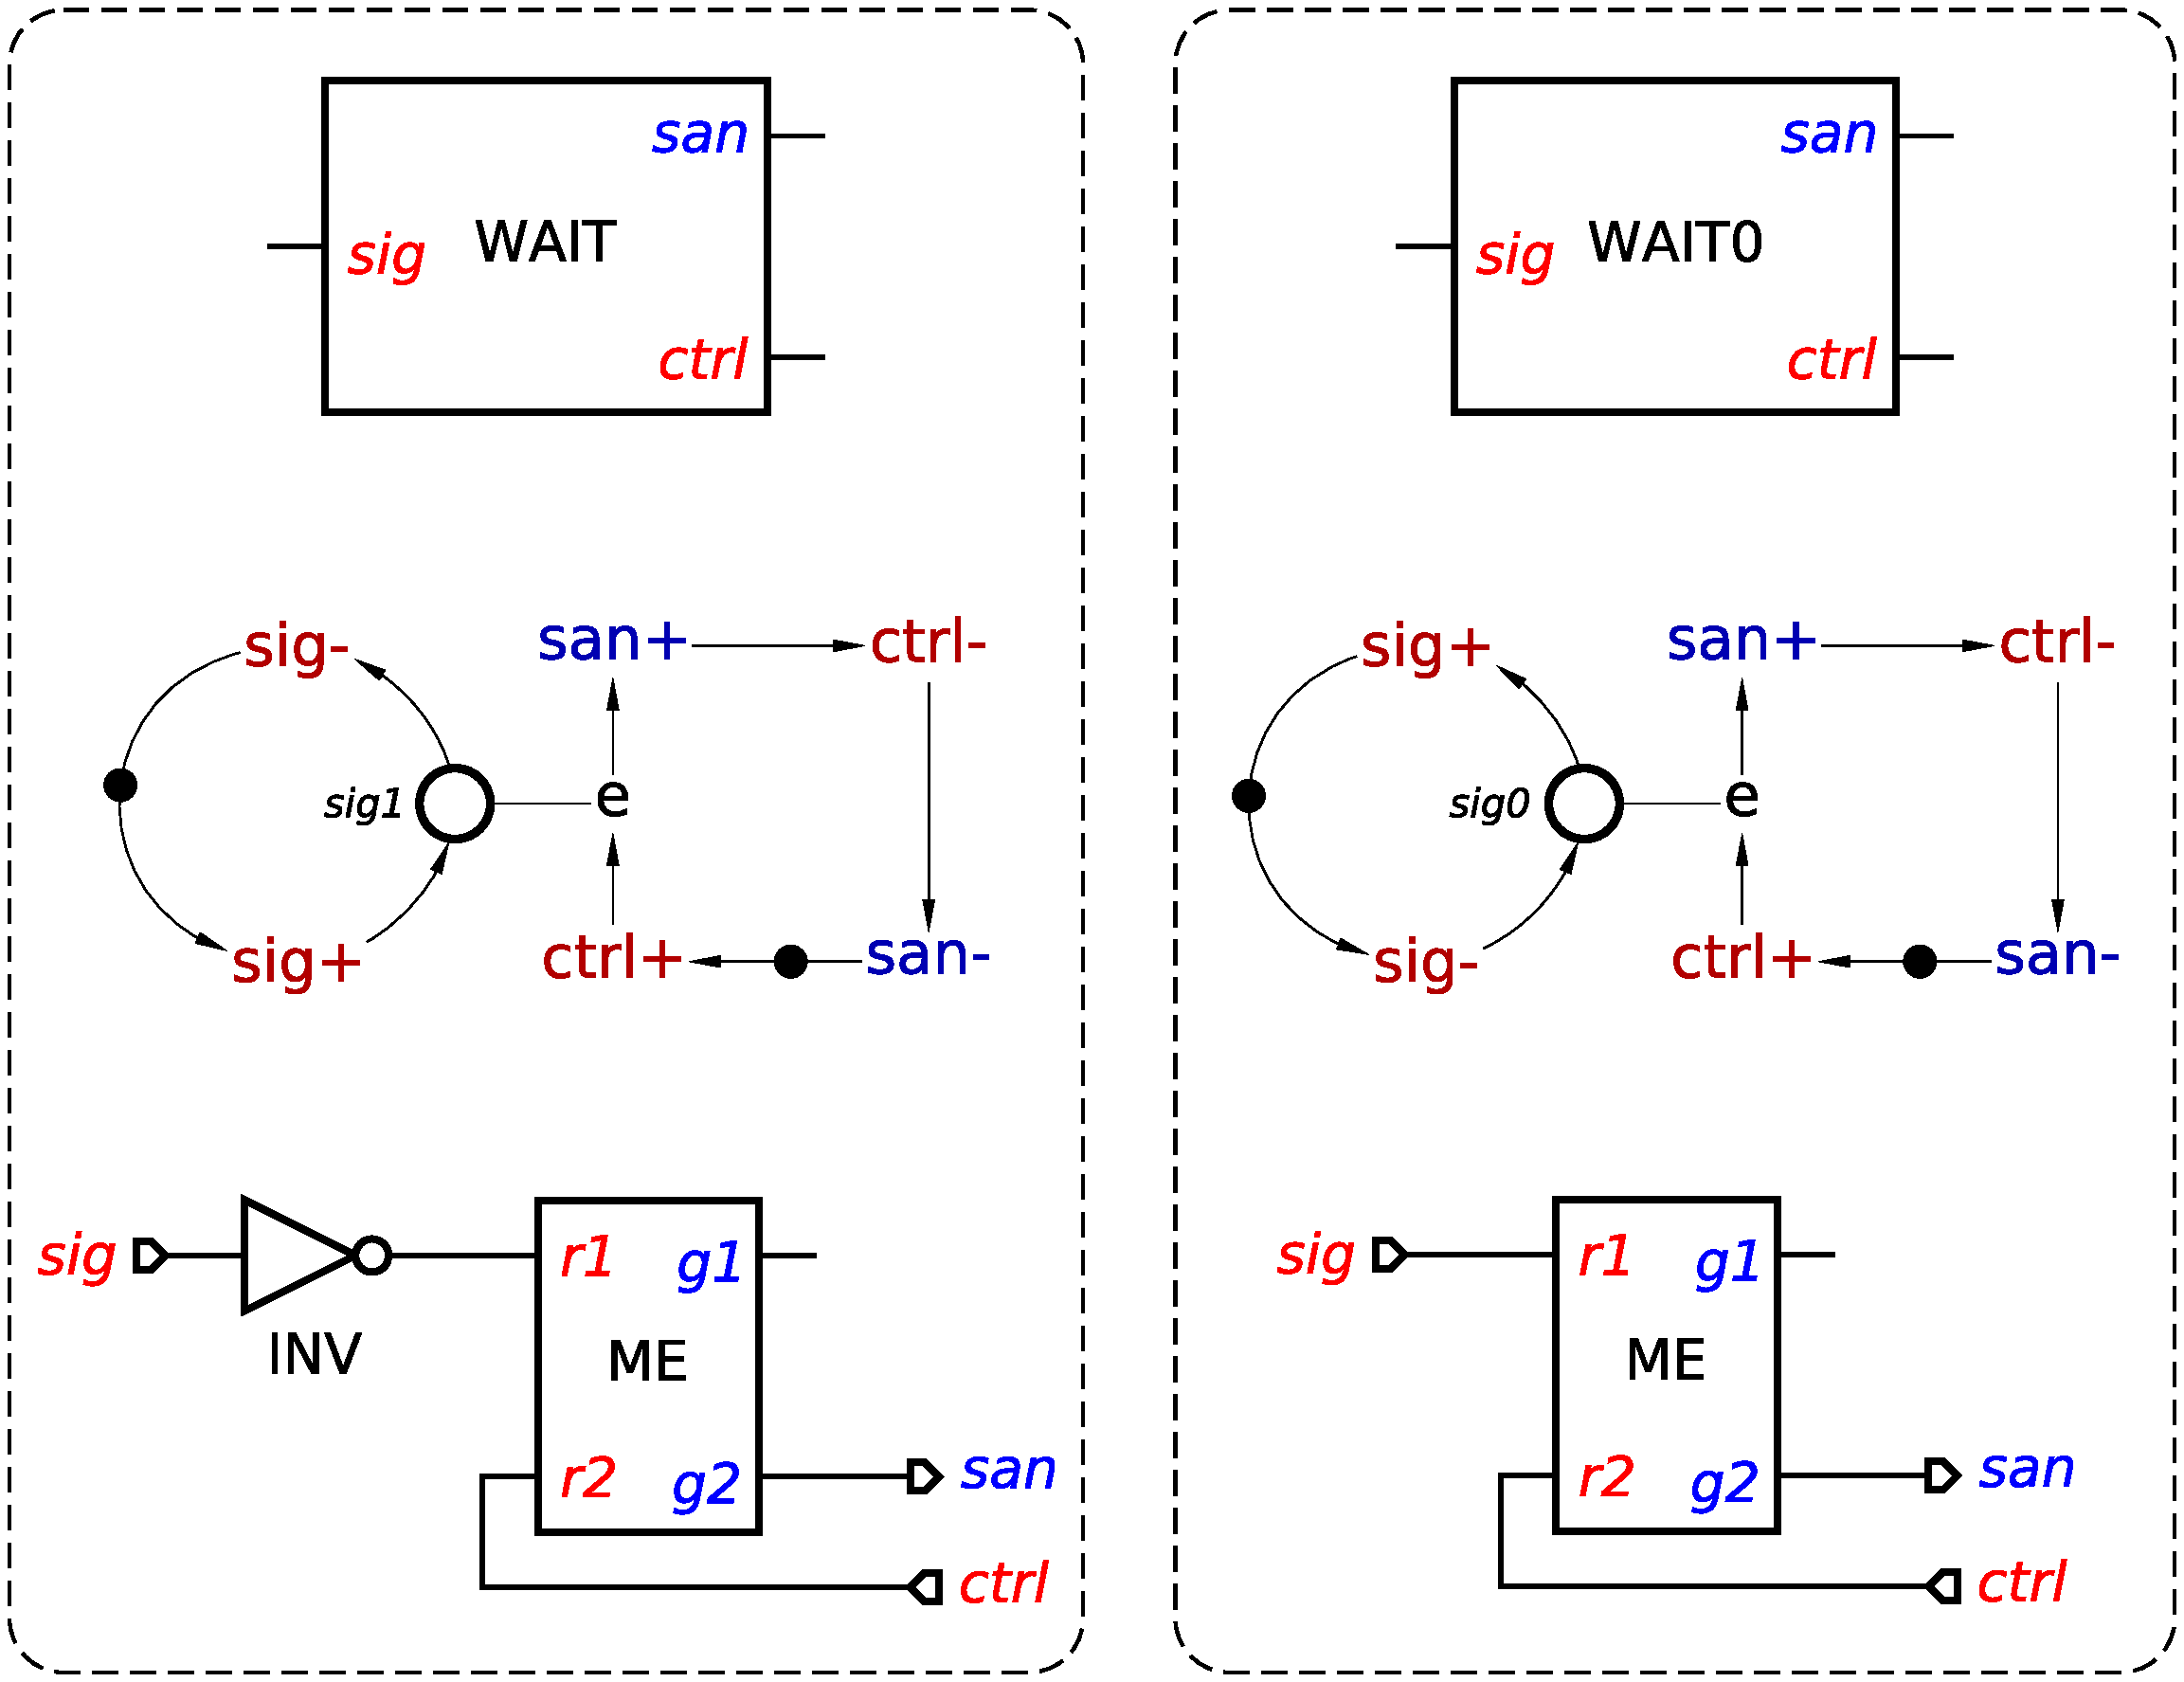
\includegraphics[scale=0.23]{fig/WAIT.pdf}
    \caption{\textsf{WAIT} and \textsf{WAIT0}: block diagram,
    specification and implementation.}
    \label{fig:wait}
\end{center}
\end{figure}

The implementation is based on the \emph{mutual-exclusion (ME)
element}~\cite{2008_kinniment_synchronisation}, which is well-known and extensively
studied by the asynchronous circuit design community.

\textsf{WAIT} is a fundamental synchronisation primitive that is used for
implementing other, more sophisticated components presented in this paper.
The symmetric version of the element that waits for the input to become low is
called \textsf{WAIT0}; its top-level block diagram, the STG specification and
the implementation are shown in Fig.~\ref{fig:wait}(right).

\subsection{\textsf{RWAIT} and \textsf{RWAIT0}}

\begin{figure*}
\begin{center}
    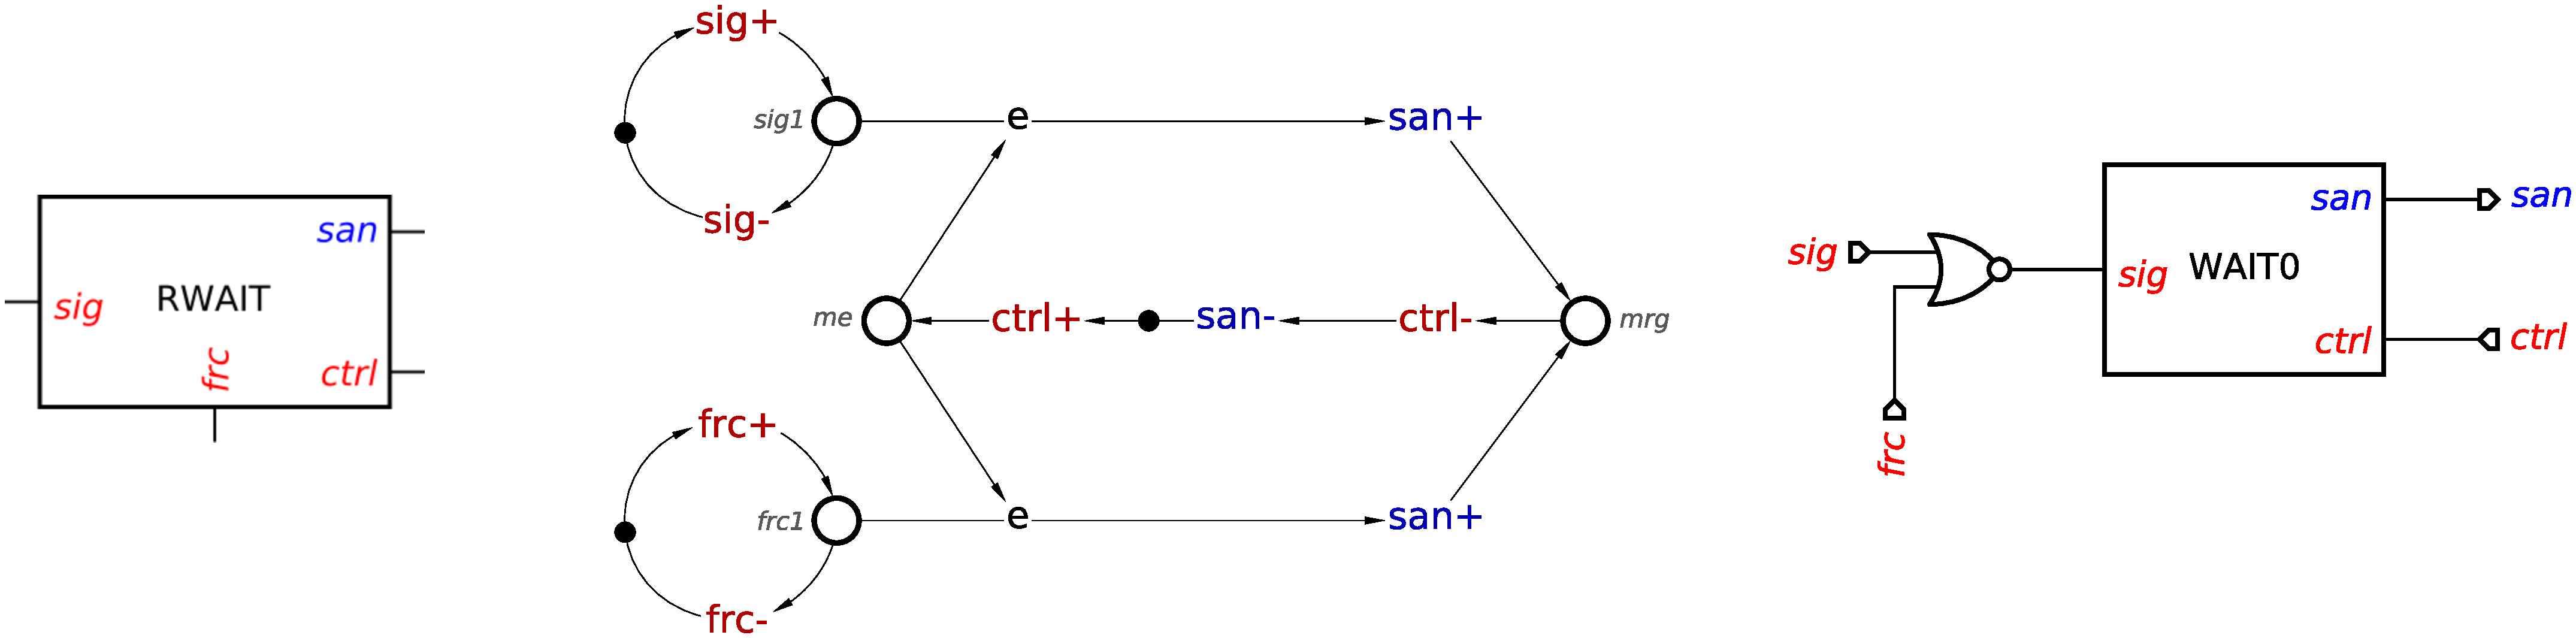
\includegraphics[scale=0.23]{fig/RWAIT.pdf}
    \caption{\textsf{RWAIT}: block diagram, specification and implementation.}
    \label{fig:rwait}
\end{center}
\end{figure*}

\textsf{RWAIT} and \textsf{RWAIT0} are modifications of the \textsf{WAIT} and \textsf{WAIT0}
elements, respectively, with a possibility to persistently cancel the waiting request. This
is useful when the input is no longer expected to change or the change is no longer relevant
for the asynchronous controller, and hence the output handshake needs to be released.

The top-level diagram of \textsf{RWAIT} is shown in Fig.~\ref{fig:rwait}. The additional input
\textsf{frc} can be used to force the reset of the output handshake in the waiting mode. The
STG specification highlights the fact that the transition \textsf{san+} can be caused either by
\textsf{sig+} or \textsf{frc+}. The implementation reflects the resulting
OR-causality~\cite{1996_yakovlev_or}: inputs \textsf{sig} and \textsf{frc} are simply combined
via a NOR gate, whose output is synchronised with the asynchronous handshake \textsf{ctrl/san}
using the \textsf{WAIT0} element.

The \textsf{RWAIT0} element is implemented analogously.

\subsection{\textsf{WAIT01} and \textsf{WAIT10}}

\textsf{WAIT01} and \textsf{WAIT10} elements wait for a rising or falling edge of the input
signal, respectively. Note, this is subtly different from waiting for high or low input value,
e.g. a signal can be initially low, and to generate a falling edge event it must first go high.

\begin{figure}
\begin{center}
    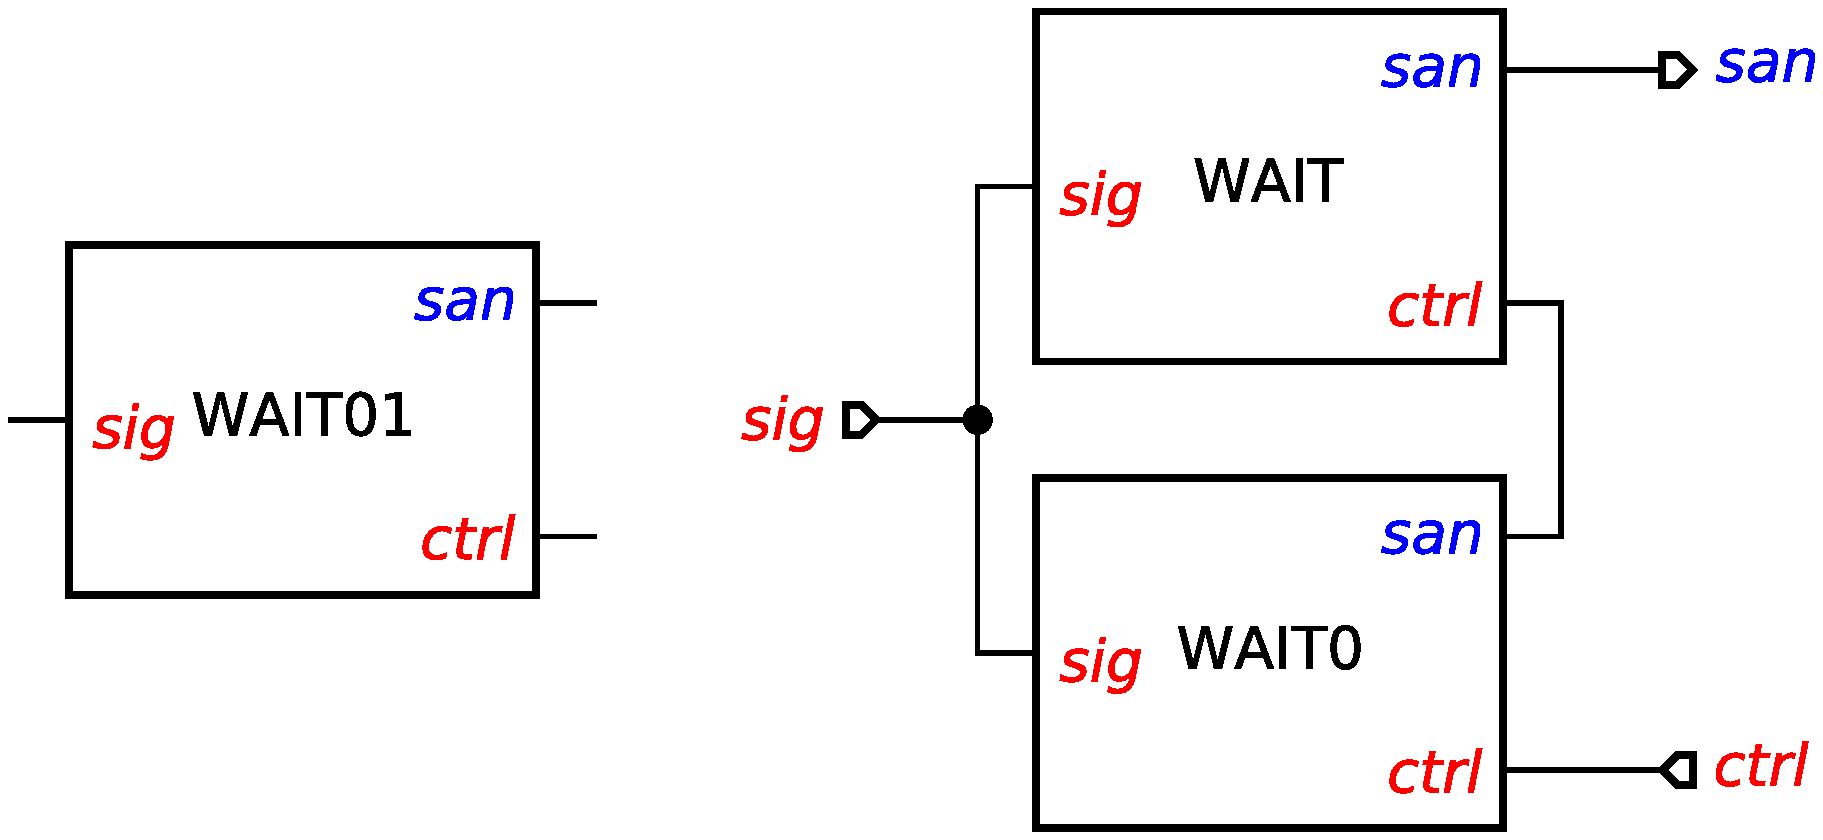
\includegraphics[scale=0.23]{fig/WAIT01.pdf}
    \caption{\textsf{WAIT01}: block diagram and implementation.}
    \label{fig:wait01}
\end{center}
\end{figure}

\subsection{\textsf{WAIT2}}
\textsf{WAIT2} is a combination of \textsf{WAIT} and \textsf{WAIT0} elements:
it uses a 2-phase output handshake, waiting for high and low input values, one after
the other.

\begin{figure}
\begin{center}
    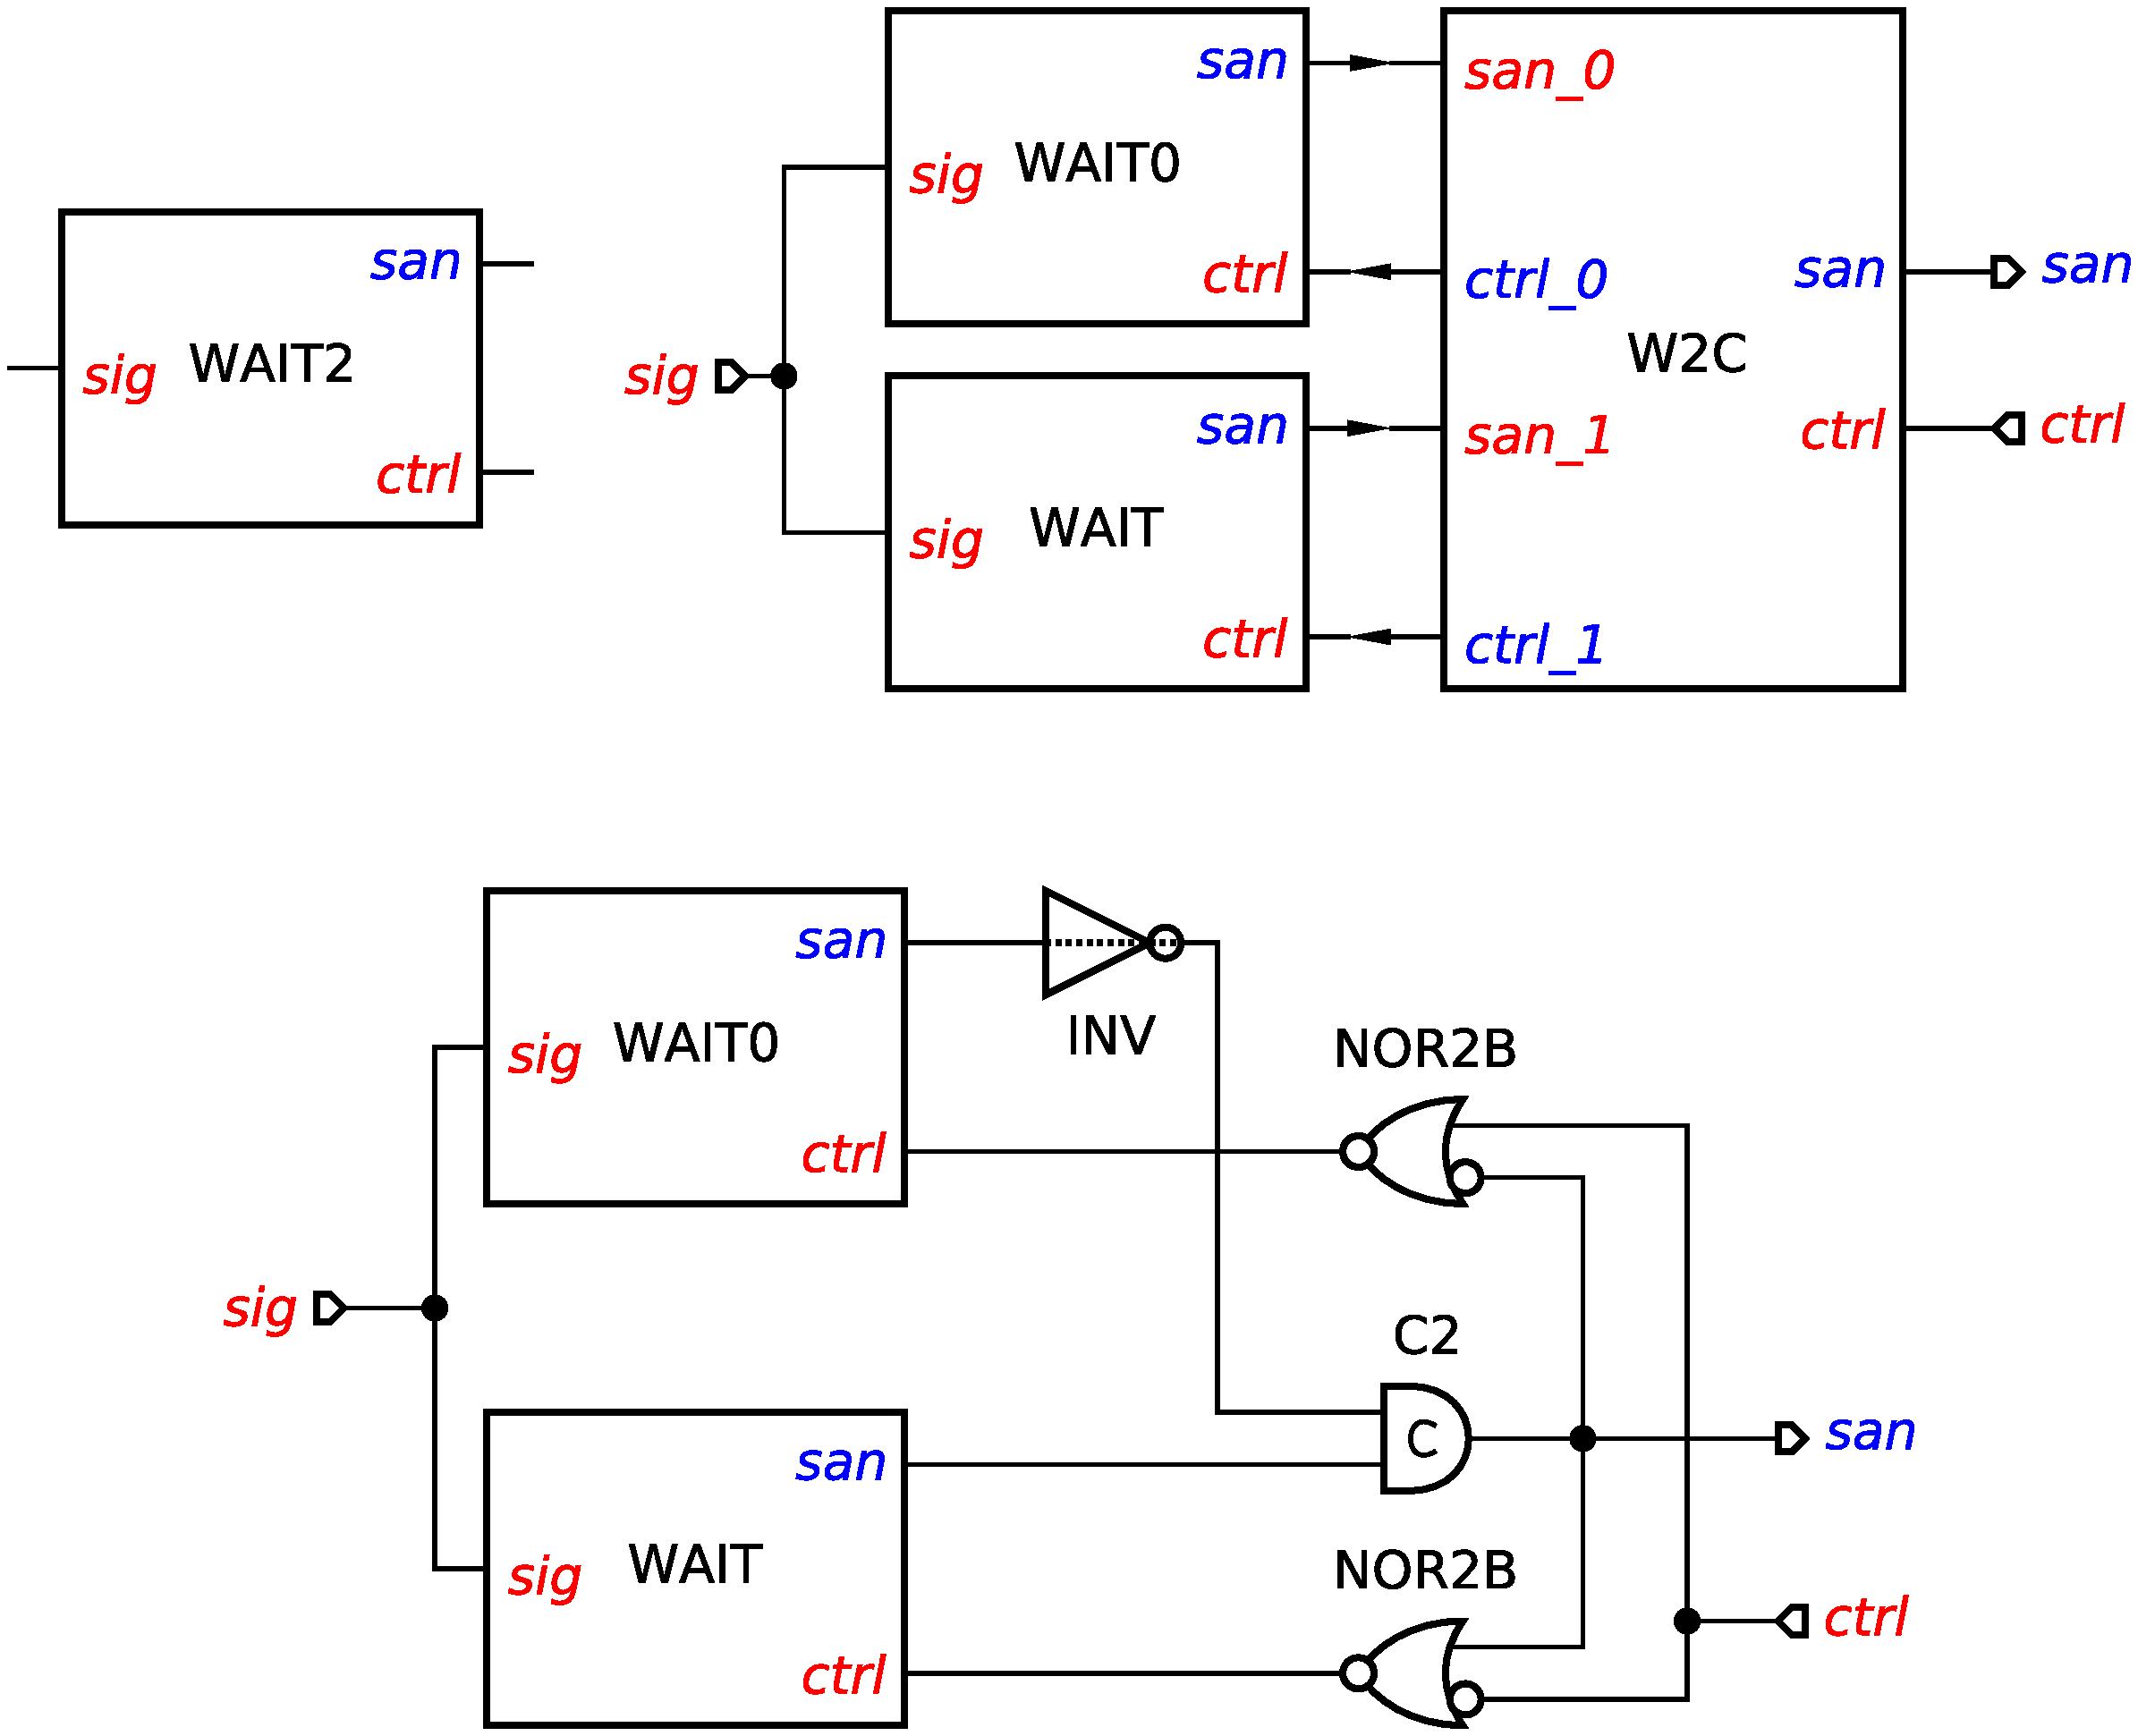
\includegraphics[scale=0.23]{fig/WAIT2.pdf}
    \caption{\textsf{WAIT2}: block diagram and conceptual design (top left and right),
    and implementation (bottom).}
    \label{fig:wait2}
\end{center}
\end{figure}

\section{Decision-making primitives}

This section presents a family of \emph{decision-making} components that perform
non-trivial event arbitration and coordination tasks and rely on the previously
introduced synchronisation primitives.

\subsection{WAITX}
\subsection{WAITX2}
\subsection{SAMPLE}
\subsection{OM}

% \begin{figure}[h!]
% \begin{center}
%   \includegraphics[width=0.84\linewidth]{FIG/ope-chip.pdf}
%   \vspace{-3mm}
%   \caption{Resiliency of asynchronous control under unstable voltage.}
%   \label{fig:voltage-resiliency}
% \end{center}
% \vspace{-7mm}
% \end{figure}

\section{Conclusions}

\section*{Acknowledgements}

\bibliographystyle{unsrt}
\bibliography{publications}

\end{document}
